\documentclass[tikz,pgfplots]{standalone}

\usepackage{tikz}
\usepackage{pgfplots}

\pgfplotsset{compat=1.15}
\usetikzlibrary{calc,positioning}


\tikzset{point/.style={draw,circle,fill=black,minimum size=8pt,
inner sep=0pt, outer sep=0pt}}


\begin{document}

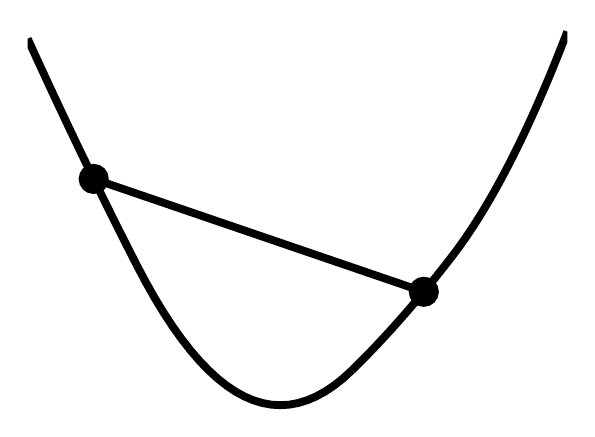
\begin{tikzpicture}
%   \begin{axis}[xmin=-0.44,xmax=0.5,line width=1mm,axis lines=none]
%     \addplot [domain=-0.44:-0.25] {8*x*(2*x-5)/10 - 0.5};
%     \addplot [domain=-0.25: 0.125] {4*3*4*x^2/5};
%     \addplot [domain= 0.125: 0.30] {8*x*(10*x+8)/35 - 4/35};
%     \addplot [domain= 0.30: 0.50] {8*x*(10*x-2)/10 + 2/5};
%     \draw (-0.325,0.969) -- (0.25,0.485714) node[point,at start] {} node[point,at end] {};
%   \end{axis}
  \begin{axis}[xmin=-0.44,xmax=0.5,line width=1mm,axis lines=none]
    \addplot [domain=-0.44:-0.25] {8*x*(2*x-5)/10 - 0.5};
    \addplot [domain=-0.25: 0.125] {4*3*4*x^2/5};
    \addplot [domain= 0.125: 0.30] {8*x*(10*x+8)/35 - 4/35};
    \addplot [domain= 0.30: 0.50] {8*x*(10*x-2)/10 + 2/5};
    \draw (-0.325,0.969) -- (0.25,0.485714) node[point,at start] {} node[point,at end] {};
  \end{axis}
\end{tikzpicture}

\end{document}